This section describes the overall design of our system, first with a system overview and then with more in depth information about our tabs.
\subsection{How the web application works}
%figure x5
\begin{figure}[h]
\centering
\includegraphics[width=0.8\textwidth]{web_system_backboneWebapp.png}
\caption{\label{fig:web_system_backboneWebapp}A general build of a backbone web app.}
\end{figure}

\refer{fig:web_system_backboneWebapp} shows how the web application works in general. There is a user that interacts with a browser. A browser renders the DOM (Document Object Model, a convention for representing and interacting with objects in HTML) of the web application. How it does this is up to the browser. Different browsers might display it differently. The web app is based on the MVC pattern, but with the controller merged into the view and with a component called \textit{Collection} being introduced. A collection is simply a ordered set of models. Models and collections will talk to the server to update themselves. Out of the components that go into this figure, we are in charge of (and only capable of) changing a few of these; \class{View}, \class{Template}, \class{Collection} and \class{Model}. See \textit{Backbone} in section \ref{sec:web_frame} more information.

\begin{example}
In the web app, there is a collection called \class{Experiments} which contains a set of \class{Experiment} models. Each of these models contains info about a specific experiment (for example, the name of the experiment and which files and annotations are incluced in it). The collection will retrieve experiments from the server and update itself with a simple call to its \class{fetch()} method. After this, the collection is synced with the server data.
\end{example}

\subsection{System overview}
%figure 2
\begin{figure}[h]
\centering
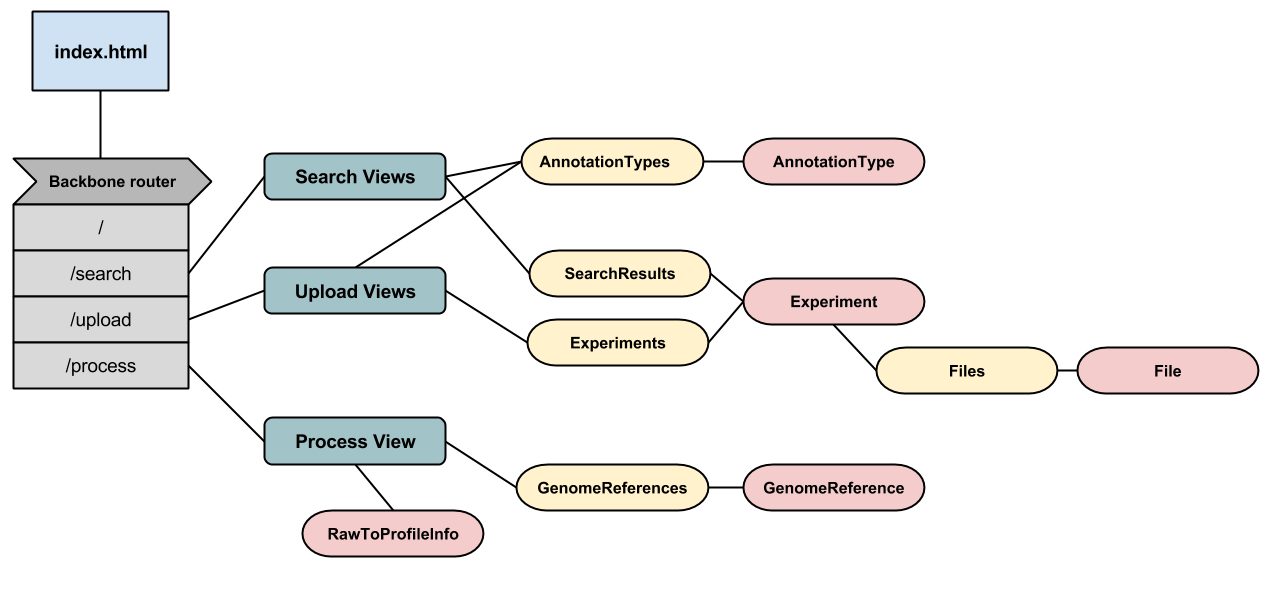
\includegraphics[width=1\textwidth]{web_system_overview.png}
\caption{\label{fig:web_system_overview}Overview of the relations between the different Javascript prototypes in the system.}
\end{figure}

The web app is divided into the parts \class{Misc}, \class{Views}, \class{Collections} and \class{Models}. In \refer{fig:web_system_overview}, an overview of the system is shown. The views are the parts in green, the collections the parts in yellow and the models the parts in red. 

\begin{example}
In \refer{fig:web_system_overview}, the collection \class{Files} contains a set of \class{File} models. The model \class{Experiment} contains a \class{Files} collection. An \class{Experiment} model may be used by the collections \class{SearchResult} and \class{Experiments}.
\end{example}

The parts in grey represent the \textit{router} which belongs in the \class{Misc} category. It is responsible for rerouting links. This is done mainly when the user wants to go to another webpage by clicking a link. The router is ``clever'', however, and does not need to load a whole web page whenever a rerouting is triggered - instead it only loads the necessary parts of the new web page.

\begin{example}
When a user clicks the \textit{search} tab, the router navigates to \url{/search}. But instead of loading the whole \url{/search} on top of the page we are currently on, the router will keep the old navigation bar, open the search tab alone and put the search tab below the already existing navigation bar.
\end{example}

The \class{Misc} category also holds the \class{main.js}, which is in charge of setting up and starting the app. The views are responsible for the user interface, displaying information and handling events. The collections and models are responsible for holding the data.

\subsection{Log in}
Log in has a single view that is a \textit{modal}, meaning that it is not a full page like the tabs but a pop-up that appears over the entire main view when a user enters the page.

\label{sec:web_search}
\subsection{Search}
The search tab has three views that together make up the \class{Search Views} as they have been denoted in \refer{fig:web_system_overview}. When searching for data, the models and collections will update themselves to contain the new annotations, experiments and files pertaining to that particular search, so the search views can display them. Once new data has been retrieved, the user can perform a number of actions on the displayed experiments and files. 

\begin{example}
When searching for experiments, they and their contained files will be displayed. The user may choose to delete a file by marking it and then click a delete button. If this happens, the \class{Search Views} will receive the event and tell the model of the marked file to destroy itself. The model will then send a delete request to the server and disappear.
\end{example}

 
%figure bla bla/lalalallala
\begin{figure}[h]
\centering
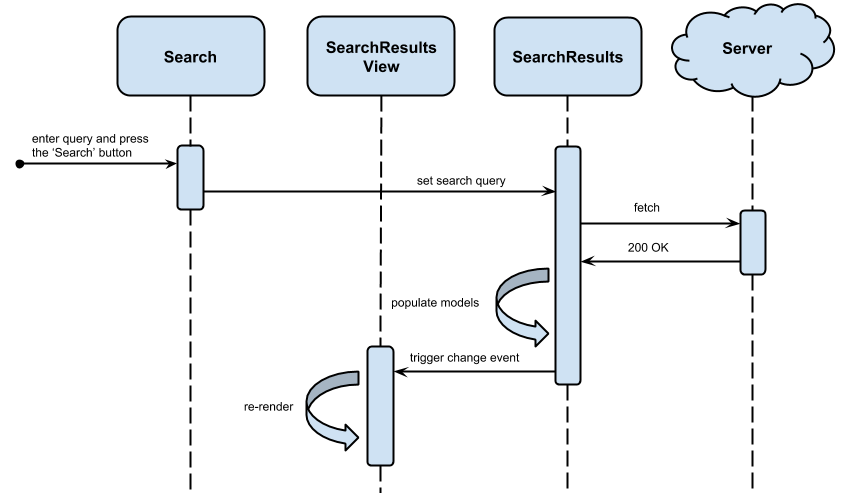
\includegraphics[width=1\textwidth]{web_system_sequenceDiagram.png}
\caption{\label{fig:web_system_sequenceDiagram}a sequence diagram showing what happens when a user enters a valid search query and results are fetched.}
\end{figure}

In \refer{fig:web_system_sequenceDiagram} is a simple sequence diagram for the search tab. If a user enters a query in the search field and then presses the search button, the \class{Search} view will update the \class{SearchResults} collection to have a new query. Once \class{SearchResults} has a new query, it will try to fetch search results corresponding to the query from the server. If successful, new experiment models for every experiment retrieved will be created and set in the \class{SearchResults} collection. \class{SearchResults} then triggers a ``change event'' that \class{SearchResultsView} listens to. When that event occurs, \class{SearchResultsView} knows that \class{SearchResults} has been changed, and rerenders itself.

\subsection{Upload}
The upload tab has three views, that together make up the ``Upload Views'' as we have denoted them in \refer{fig:web_system_overview}. Unlike search (see section \ref{sec:web_frame}) that uses experiment and file models to retrieve information about experiments and files, upload uses the same models to create new experiments and files. To do this, it needs to be aware of what annotations are available, so it uses an annotation type collection to retrieve the current annotations offered when a user wants to create a new experiment.

\subsection{Process} 
Process consists of two views that are reached either through the process
tab in the main navigation bar or through the process button in the search view
that allows the user to search for experiments prior to entering the process
view. Process also has collections and models to store and send data necessary 
for a process, like genome releases available for the chosen species of an 
experiment.

The view reached through the tab is simply a textfield where you can enter an
experiment name and a button which allows you to proceed to the process view
for that experiment, which is exactly the same thing that happens when marking
an experiment in the search view and pressing the process button there.

The process view is at first only a dropdown list where any process step can
be chosen and added to the view by pressing the add button. Similarly, to each 
process step, a line can be added using the + button, which represents one run
of that process step. Adding more than one line to one step allows simultaneous
processing, but should any infile depend on an outfile a new process step of the
same sort must be created below.